\section{Introduction}
\begin{figure}[ht]
  \centering
  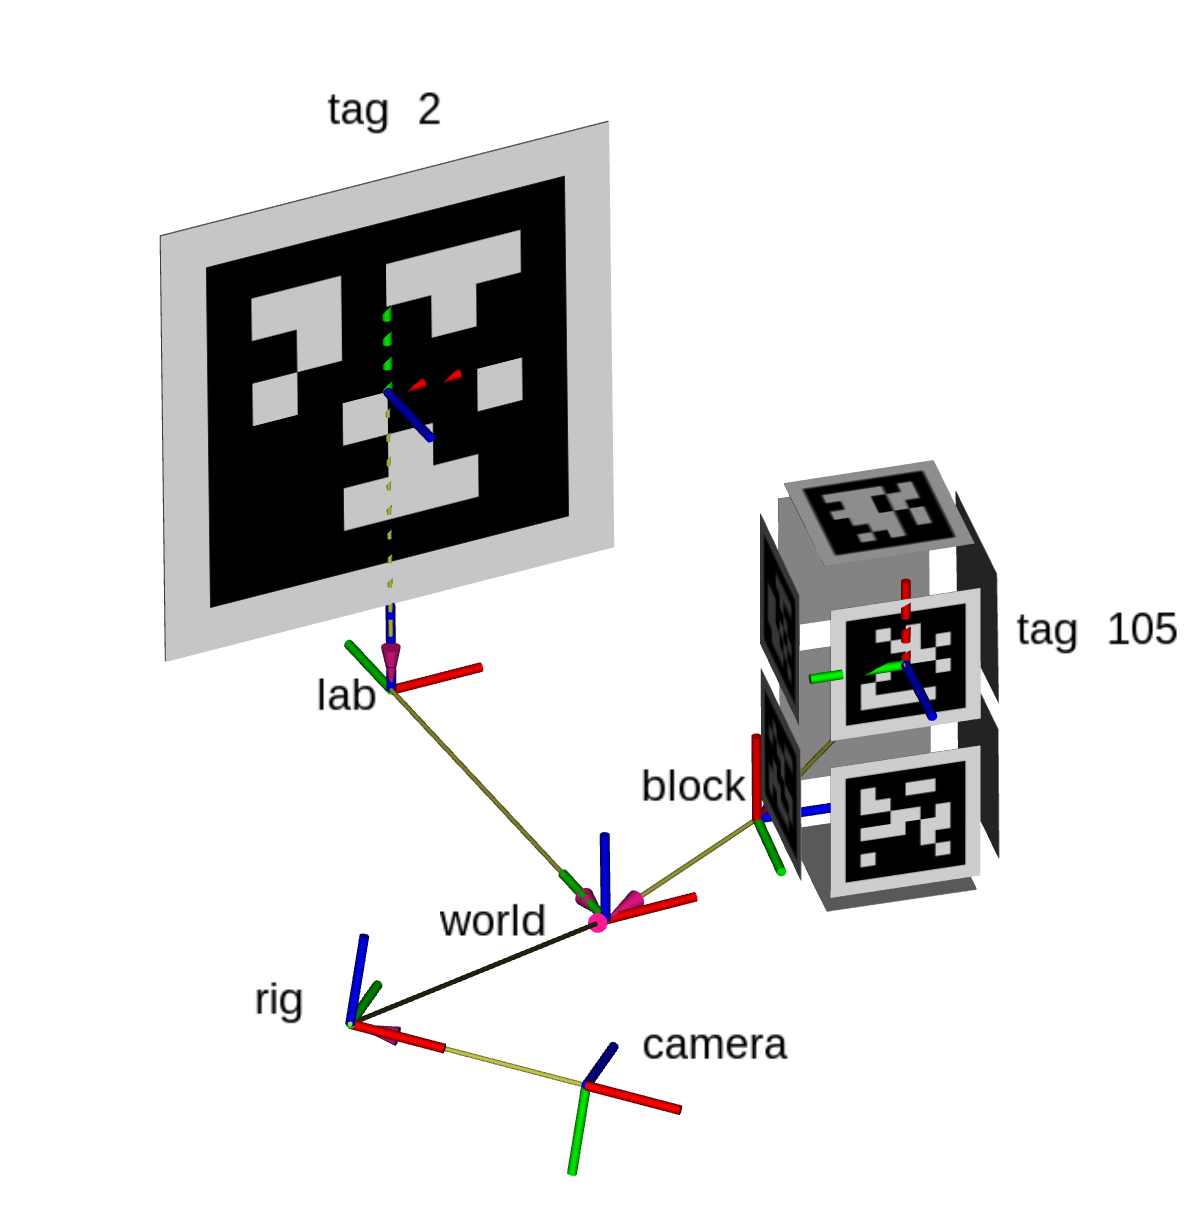
\includegraphics[width=0.8\columnwidth]{scene_with_block.png}
  \caption{Single-camera TagSLAM scene with dynamic ``rig'' and ``block''
    bodies, and a static ``lab'' body.}
  \label{fig:scene_with_block}
\end{figure}

Accurate and robust Simultaneous Localization And Mapping (SLAM)
algorithms are arguably one of the corner pieces for building
autonomous systems. For this reason, SLAM has been studied extensively
since the 1980s \cite{cadena2016}. 
In a nutshell, SLAM methods take sensor data such as camera images as
input and extract easily recognizable features (``landmarks''). The
landmarks are entered into a map such that when the same landmark is
detected again later, the observer's pose can be determined by
triangulation. In graph based SLAM, a nonlinear optimizer such as
GTSAM \cite{kaess2011} is used to simultaneously optimize the pose of
the observer and the location of the landmarks, given the sensor
measurements.

Much research effort \cite{cadena2016} has gone into solving the
hard aspects of SLAM. One of them is recognizing previously seen
landmarks (''loop closure''). This is often difficult if landmarks are
observed from a different viewpoint, or under different lighting
conditions. The other is maintaining a map of landmarks. To limit memory 
consumption and achieve fast retrieval, landmarks must be at some
point discarded, efficient retrieval databases must be updated and
queried, adding considerable complexity \cite{murartal2017}. If loop
closure fails, the estimated camera pose starts to drift, which is a
well-known problem with local-map-only algorithms such as
visual-inertial odometry (VIO).

In many situations, and in particular for laboratory experiments these
problems can be sidestepped with a mild intervention to the 
environment. By placing visual fiducial markers such as the
popular AprilTags \cite{wang2016} in a scene, one can create a small
set of artifical landmarks, typically numbering less than 100. The
TagSLAM framework presented in this paper is designed for such a situation.
With only a few landmarks to consider, memory and retrieval speed are
no longer critical, and loop closure is 
guaranteed once a tag is successfully decoded by the AprilTag
library. If one or more tags are visible at all times, then TagSLAM
can perform both tracking and loop closure.

But more importantly, tags permit the introduction of geometric
constraints that have been observed by other means. For instance, markers
can be placed inside a building at coordinates that are known because
a highly accurate building plan is available
\cite{pfrommer2017}. Another alternative is measuring the locations
of select tags with a laser distance measuring tool. When a measured
marker is later recognized by the moving camera, it will pull the
trajectory to the reference location. As we demonstrate in the
experimental section, this can augment existing SLAM or
VIO methods. By utilizing well-known tags in a few places, and
ubiquitous but anonymous feature points elsewhere, one can leverage
the advantages of both approaches.

Even though tag based SLAM is much simpler than general SLAM, some
remaining difficulties are addressed in this paper. Since TagSLAM
utilizes GTSAM  \cite{kaess2011}, a graph based non-convex optimizer, care must be taken
to properly initialize all starting values. A bad initial value can
cause the optimizer to fail or to converge to a local minimum. In the
present work we give a detailed description of how we achieve robust
initialization to make TagSLAM a tool that can be applied to a wide range of
real-world situations without parameter tuning.

It is worthwhile noting that SLAM is a rather general algorithm, and
therefore can solve several related, simpler problems as well. If for
example the camera pose is known, one can estimate the pose of the
landmarks. Likewise, if a map of the landmarks is known, the camera
pose can be inferred. TagSLAM inherits all of this flexibility. In
contrast to traditional SLAM packages however, where moving landmarks
are filtered out, TagSLAM can explicitly model and track multiple
objects that have tags attached to them. This means TagSLAM can also
be used for pose estimation of objects other than cameras, as shown in
Fig. \ref{fig:scene_with_block}. In fact, TagSLAM has been deployed for
the University of Pennsylvania's Smart Aviary project in a scenario
where {\em all} cameras are static. This is not directly possible with any SLAM
package that we are aware of.

TagSLAM's robustness and
availability as an open-source ROS \cite{quigley2009} package make it
particularly accessible for researchers new to robotics. It is now
being used at the University of Pennsylvania's GRASP lab for extrinsic camera calibration with
non-overlapping views, loop closure on visual-inertial odometry
benchmarks, tag mapping, object pose estimation, and more. TagSLAM is
also employed in a forthcoming project by the University of Michigan's
DASC laboratory.
